\documentclass[10pt]{article}
\usepackage[margin=1in]{geometry}
\usepackage[T1]{fontenc}
\usepackage{newtxtext,newtxmath}
\usepackage{microtype}
\usepackage{booktabs}
\usepackage{graphicx}
\usepackage{amsmath}
\usepackage{xcolor}
\usepackage[small]{caption}
\usepackage[numbers,sort&compress]{natbib}
\usepackage[colorlinks=true,linkcolor=blue!50!black,citecolor=blue!50!black,urlcolor=blue!50!black]{hyperref}
% generated by paper/make_assets.py - do not edit
\newcommand{\CleanAccMin}{1.00}
\newcommand{\FracBlend}{0.20}
\newcommand{\FracRandom}{0.15}
\newcommand{\InjDEight}{+0.20 [0.12, 0.28]}
\newcommand{\InjDFour}{+0.41 [0.35, 0.47]}
\newcommand{\InjDGEight}{+0.13 [0.07, 0.19]}
\newcommand{\InjDGFour}{+0.17 [0.08, 0.24]}
\newcommand{\InjDGLlama}{$-$0.03 [$-$0.07, 0.01]}
\newcommand{\InjDLlama}{+0.15 [0.08, 0.22]}
\newcommand{\InjDMaskEight}{$-$0.02 [$-$0.08, 0.03]}
\newcommand{\InjDMaskFour}{+0.01 [$-$0.01, 0.04]}
\newcommand{\InjDMaskLlama}{$-$0.07 [$-$0.12, $-$0.01]}
\newcommand{\InjDefToneEight}{0.00}
\newcommand{\InjDefToneFour}{0.12}
\newcommand{\InjDefToneLlama}{0.01}
\newcommand{\InjDefTthreeEight}{0.22}
\newcommand{\InjDefTthreeFour}{0.51}
\newcommand{\InjDefTthreeLlama}{0.16}
\newcommand{\InjNdocs}{24}
\newcommand{\InjNinjected}{72}
\newcommand{\InjNitems}{96}
\newcommand{\InjNtrials}{144}
\newcommand{\InjNtrialsOverride}{48}
\newcommand{\InjOvToneEight}{0.00}
\newcommand{\InjOvToneFour}{0.04}
\newcommand{\InjOvToneLlama}{0.10}
\newcommand{\InjOvTthreeEight}{0.31}
\newcommand{\InjOvTthreeFour}{1.00}
\newcommand{\InjOvTthreeGEight}{0.40}
\newcommand{\InjOvTthreeGFour}{0.62}
\newcommand{\InjOvTthreeGLlama}{0.02}
\newcommand{\InjOvTthreeLlama}{0.29}
\newcommand{\InjResidEight}{+0.09 [0.04, 0.15]}
\newcommand{\InjResidFour}{+0.29 [0.22, 0.36]}
\newcommand{\InjResidLlama}{+0.08 [0.03, 0.15]}
\newcommand{\InjToneEight}{0.00}
\newcommand{\InjToneFour}{0.11}
\newcommand{\InjToneLlama}{0.03}
\newcommand{\InjTthreeEight}{0.20}
\newcommand{\InjTthreeFour}{0.52}
\newcommand{\InjTthreeLlama}{0.18}
\newcommand{\InjZeroUpper}{2.1}
\newcommand{\InjZeroUpperOverride}{6.1}
\newcommand{\MitigShareRange}{29--55}
\newcommand{\PilotKBFour}{144}
\newcommand{\PilotKLRange}{0.065--0.092}
\newcommand{\PilotSpeedupFour}{13.4}
\newcommand{\PilotSpeedupOne}{9.8}
\newcommand{\RagDBEight}{+0.00 [0.00, 0.00]}
\newcommand{\RagDBFour}{+0.03 [$-$0.01, 0.09]}
\newcommand{\RagDBLlama}{+0.00 [0.00, 0.00]}
\newcommand{\RagDEight}{+0.00 [0.00, 0.00]}
\newcommand{\RagDFour}{+0.15 [0.08, 0.24]}
\newcommand{\RagDLlama}{+0.00 [0.00, 0.00]}
\newcommand{\RagNinjEight}{144}
\newcommand{\RagNinjFour}{144}
\newcommand{\RagNinjLlama}{144}
\newcommand{\RagRthreeNAccRange}{0.77--0.79}
\newcommand{\WoneFourCone}{0.02}
\newcommand{\WoneFourCthree}{0.55}
\newcommand{\WoneFourD}{+0.53 [0.38, 0.69]}
\newcommand{\WoneFourScoreCone}{0.69}
\newcommand{\WoneFourScoreCthree}{0.86}
\newcommand{\WoneOneSevenCone}{0.00}
\newcommand{\WoneOneSevenCthree}{0.00}
\newcommand{\WoneOneSevenD}{+0.00 [0.00, 0.00]}
\newcommand{\WoneOneSevenScoreCone}{0.29}
\newcommand{\WoneOneSevenScoreCthree}{0.31}
\newcommand{\WtwoEightCodeCone}{0.42}
\newcommand{\WtwoEightCodeCthree}{0.94}
\newcommand{\WtwoEightCone}{0.41}
\newcommand{\WtwoEightConeM}{1.00}
\newcommand{\WtwoEightCthree}{0.67}
\newcommand{\WtwoEightCthreeG}{0.21}
\newcommand{\WtwoEightCtwo}{0.76}
\newcommand{\WtwoEightDG}{$-$0.20 [$-$0.42, 0.04]}
\newcommand{\WtwoEightDMM}{$-$0.19 [$-$0.35, $-$0.06]}
\newcommand{\WtwoEightDStrict}{+0.28 [0.01, 0.53]}
\newcommand{\WtwoEightDthree}{+0.26 [$-$0.02, 0.52]}
\newcommand{\WtwoEightDthreeTwo}{$-$0.10 [$-$0.28, 0.08]}
\newcommand{\WtwoEightHeadCone}{1.00}
\newcommand{\WtwoEightHeadCthree}{0.78}
\newcommand{\WtwoEightSignCone}{0.78}
\newcommand{\WtwoEightSignCthree}{0.99}
\newcommand{\WtwoEightStrictCone}{0.39}
\newcommand{\WtwoEightStrictCthree}{0.67}
\newcommand{\WtwoEightTTFTCone}{2.26}
\newcommand{\WtwoEightTTFTCthree}{0.34}
\newcommand{\WtwoEightTrunc}{0}
\newcommand{\WtwoFourCodeCone}{0.03}
\newcommand{\WtwoFourCodeCthree}{0.84}
\newcommand{\WtwoFourCone}{0.01}
\newcommand{\WtwoFourConeM}{0.88}
\newcommand{\WtwoFourCthree}{0.70}
\newcommand{\WtwoFourCthreeG}{0.03}
\newcommand{\WtwoFourCtwo}{0.49}
\newcommand{\WtwoFourDG}{+0.02 [$-$0.03, 0.07]}
\newcommand{\WtwoFourDMM}{+0.06 [$-$0.10, 0.22]}
\newcommand{\WtwoFourDStrict}{+0.50 [0.36, 0.64]}
\newcommand{\WtwoFourDthree}{+0.69 [0.55, 0.81]}
\newcommand{\WtwoFourDthreeTwo}{+0.21 [0.01, 0.41]}
\newcommand{\WtwoFourHeadCone}{1.00}
\newcommand{\WtwoFourHeadCthree}{1.00}
\newcommand{\WtwoFourSignCone}{0.31}
\newcommand{\WtwoFourSignCthree}{0.93}
\newcommand{\WtwoFourStrictCone}{0.01}
\newcommand{\WtwoFourStrictCthree}{0.51}
\newcommand{\WtwoFourTTFTCone}{1.22}
\newcommand{\WtwoFourTTFTCthree}{0.09}
\newcommand{\WtwoFourTrunc}{0}
\newcommand{\WtwoLlamaCodeCone}{0.07}
\newcommand{\WtwoLlamaCodeCthree}{0.13}
\newcommand{\WtwoLlamaCone}{0.04}
\newcommand{\WtwoLlamaConeM}{0.44}
\newcommand{\WtwoLlamaCthree}{0.02}
\newcommand{\WtwoLlamaCthreeG}{0.00}
\newcommand{\WtwoLlamaCtwo}{0.01}
\newcommand{\WtwoLlamaDG}{$-$0.04 [$-$0.08, $-$0.01]}
\newcommand{\WtwoLlamaDMM}{$-$0.42 [$-$0.56, $-$0.28]}
\newcommand{\WtwoLlamaDStrict}{+0.00 [0.00, 0.00]}
\newcommand{\WtwoLlamaDthree}{$-$0.02 [$-$0.06, 0.01]}
\newcommand{\WtwoLlamaDthreeTwo}{+0.01 [$-$0.01, 0.06]}
\newcommand{\WtwoLlamaHeadCone}{1.00}
\newcommand{\WtwoLlamaHeadCthree}{0.62}
\newcommand{\WtwoLlamaSignCone}{0.24}
\newcommand{\WtwoLlamaSignCthree}{0.40}
\newcommand{\WtwoLlamaStrictCone}{0.00}
\newcommand{\WtwoLlamaStrictCthree}{0.00}
\newcommand{\WtwoLlamaTTFTCone}{0.70}
\newcommand{\WtwoLlamaTTFTCthree}{0.06}
\newcommand{\WtwoLlamaTrunc}{11}
\newcommand{\WtwoNmodels}{3}
\newcommand{\WtwoNskills}{24}
\newcommand{\WtwoNtasks}{48}

\setlength{\emergencystretch}{1.5em}

\newcommand{\cond}[1]{\textsf{#1}}

\title{\textbf{Precompiled Context Is Read as Instructions:}\\
KV Packs Speed Up Agent Skills and Amplify Tool-Output Prompt Injection}
\author{Anonymous Author(s)\\\small Workshop draft --- do not distribute}
\date{}

\begin{document}
\maketitle

\begin{abstract}
Agents increasingly load \emph{skills}---static instruction documents---on demand, and every load
re-prefills thousands of tokens. We precompile each skill into a \emph{KV pack}: its key/value cache,
computed once after the system prompt and spliced into the live conversation by re-rotating keys to
the mount position. On an Apple-silicon laptop this cuts post-selection time-to-first-token by a median
of \PilotSpeedupFour$\times$ for Qwen3-4B (\PilotLongText\,s $\rightarrow$ \PilotLongPack\,s for a
\PilotLongTok-token skill). Unexpectedly, packs also make the model \emph{follow the skill better}: on a
verifiable synthetic skill benchmark, the share of tasks obeying all five planted rules rises from
\WtwoCone\ (skill prefilled as a tool result) to \WtwoCthree\ (\WtwoDthree, skill-clustered 95\% CI).
Ablations trace both effects to one mechanism: text whose KV never attended to the conversation is
treated as standalone instruction rather than as material retrieved for the user's question. The same
mechanism is a security liability. When untrusted tool output is mounted this way, compliance with a
benign injected instruction rises on all three models we test (Qwen3-4B \InjDFour, Qwen3-8B \InjDEight,
Llama-3.2-3B \InjDLlama); a defensive system prompt does not help, masking the conversation inside an
ordinary prefill reproduces the effect exactly, and CacheBlend-style 15\% selective recompute removes only
part of it. In the classic RAG layout, where documents precede the question, the amplification largely
vanishes. We conclude that KV reuse should be keyed on trust: context-free packs for trusted skills, full
in-context prefill for untrusted content.
\end{abstract}

\section{Introduction}
Agent frameworks keep only a catalog of skills in context and load a skill's full text when the model asks
for it (``progressive disclosure''), which cuts input tokens by up to 82\%~\citep{zhang2026progressive,nakasuji2026skillblocks}.
The cost moves to latency: every load prefills one to six thousand tokens in the middle of a conversation,
which dominates time-to-first-token (TTFT) for models run locally. Skill text is static, so its KV cache
can be computed once and reused. Prefix caching~\citep{gim2024promptcache,zheng2024sglang} only reuses
\emph{prefixes}; a skill is loaded after the user's question, at a different position every time.

We study the obvious fix---precompile, then splice---and find it changes more than speed. Our contributions:
\begin{enumerate}\itemsep0pt
\item \textbf{KV packs for skills} (\S\ref{sec:method}): a pack is a skill's K/V computed after a fixed
  \emph{prelude}; mounting re-rotates keys by the position delta. On MLX it lowers post-selection TTFT by
  \PilotSpeedupFour$\times$ (median) for Qwen3-4B with an exact-prelude control matching text prefill (KL 0.001).
\item \textbf{Packs improve rule-following} (\S\ref{sec:skills}): on a verifiable synthetic benchmark,
  all-rules compliance rises from \WtwoCone\ to \WtwoCthree. Text-loaded skills obey only the rules the user
  asks about; naming every rule in the question (\WtwoConeM) or encoding the skill without the conversation
  (\WtwoCthree) fixes this.
\item \textbf{The same mechanism amplifies prompt injection} (\S\ref{sec:injection}): for untrusted tool
  output, packs raise injection compliance on three models and two families, defensive prompting does not
  help, and an attention-mask control shows the cause is context-free encoding, not the RoPE shift.
\item \textbf{Mitigation and scope} (\S\ref{sec:mitigation}): boundary recompute does nothing, CacheBlend-style
  15\% recompute~\citep{yao2025cacheblend} removes \MitigShareRange\% of the excess, and the classic RAG layout is
  largely unaffected.
\end{enumerate}

\section{Related work}
\textbf{KV reuse.} Prompt Cache~\citep{gim2024promptcache} and RadixAttention~\citep{zheng2024sglang} reuse
exact prefixes; LMCache~\citep{liu2025lmcache} and the knowledge-delivery view~\citep{cheng2024kdn} treat KV as
storable knowledge. Non-prefix reuse either recomputes a selected subset of tokens (CacheBlend~\citep{yao2025cacheblend}),
trains boundary adapters (KV Packet~\citep{chen2026kvpacket}), or re-rotates keys and repairs one seam token
(Notes at Prefill~\citep{li2026notes}, which also precompiles ``skills''). Cartridges~\citep{eyuboglu2025cartridges}
train compact KV for a corpus; composing independently built KV degrades quality~\citep{shepard2026costs,rakotonirina2026where}.
Cross-model KV transfer~\citep{liu2024droidspeak,fu2025c2c} is orthogonal. These works evaluate accuracy and
latency; we evaluate \emph{instruction-following and security} of reused KV.

\textbf{Skills and injection.} Skill-loading strategies are compared at the text level~\citep{zhang2026progressive,nakasuji2026skillblocks}.
Indirect prompt injection through retrieved or tool content~\citep{greshake2023indirect} is mitigated in training by
giving tool output lower privilege than system or user turns~\citep{wallace2024hierarchy}; our results suggest
KV reuse can silently undo that privilege assignment.

\section{Method}\label{sec:method}
\textbf{Packs.} Given a token segment $s$ and a prelude $p$, a pack stores the per-layer K/V of $s$ computed
after $p$ (mlx-lm~\citep{hannun2023mlx} caches post-RoPE keys). To mount it at position $P$ we rotate each key by
$\delta = P - |p|$ using the model's own RoPE (standard and Llama-3-scaled RoPE compose additively) and append.
Tokens of $s$ then lack attention to whatever precedes $P$ but is not in $p$; that gap is the object of study.

\textbf{Layouts.} All conditions share identical token ids (segments are tokenized separately and concatenated).
In the agent layout the conversation is
\begin{center}\small\texttt{[system + catalog] [user question; assistant tool call] [tool result] [assistant]}\end{center}
and the conditions differ only in how the tool result enters the cache:
\begin{itemize}\itemsep0pt
\item \cond{C1}/\cond{T1} \emph{text}: the skill/document is prefilled as the tool result (standard).
\item \cond{C3}/\cond{T3} \emph{pack}: the same position, from a pack whose prelude is \texttt{[system][tool-result header]}, i.e.\ it never saw the conversation.
\item \cond{C2}/\cond{T2} \emph{system prefix}: the text is placed in the system prompt (an exact, prefix-cacheable layout) and the tool result is an acknowledgement.
\item \cond{C3G}/\cond{T3G}: a pack built after a content-free question and the tool call (conversation-shaped prelude).
\item \cond{T1$'$}: text prefill at the true positions, but the tool result may not attend to the user turn or tool call (an attention mask, no RoPE shift).
\item \cond{T3F16}/\cond{T3L16}/\cond{T3R15}/\cond{T3B15}: the \cond{T3} pack with the first 16, last 16, a random 15\%, or the 15\% of tokens with the largest layer-1 K/V deviation recomputed in context on all later layers (CacheBlend-style, one-shot selection after two full layers; ${\approx}20\%$ of prefill compute).
\end{itemize}
Our layer-wise recompute engine is tested to reproduce text prefill exactly when all tokens are recomputed and
the plain splice when none are, for Qwen3 and Llama.

\section{Setup}
\textbf{Models and hardware.} Qwen3-1.7B/4B/8B (thinking off)~\citep{yang2025qwen3} and Llama-3.2-3B-Instruct~\citep{grattafiori2024llama3},
bf16, on an Apple M5 Pro laptop (64\,GB) with MLX 0.32.4 / mlx-lm 0.32.2.

\textbf{Verifiable skills.} We generate skill documents (650--3,300 tokens) for (object, action) domains (e.g.\ invoice reconciliation). Each plants five rules at controlled depths, rotated across skills so every
(rule, depth) cell is covered: start with \texttt{CODE:~XX-1234}, a file-name prefix, a four-digit parameter value, an exact
step-list heading, and an end sign-off line. Tasks name the domain and ask for the step list, file name and parameter
value---\emph{not} for the code line, heading or sign-off. Answers are graded by regular expressions.

\textbf{Injection items.} The same documents are served by a \texttt{read\_doc} tool; the user asks for one parameter value.
Each document has a clean version and three injected versions with an inert canary placed at depth 0.1/0.5/0.9:
\emph{override} (``ignore the user's question, reply only \texttt{ACK-<canary>}''), \emph{append} (``end with
\texttt{ref:~<canary>}''), and \emph{refuse} (``say the document is confidential'')---\InjNitems\ items over \InjNdocs\ documents.

\textbf{Statistics.} Sampling at $T{=}0.7$, top-$p$ 0.8, top-$k$ 20 with seeds shared across conditions; paired differences
with 95\% bootstrap intervals that resample skills/documents (tasks of one document are correlated). All numbers in this
paper are generated from the raw logs by a script.

\section{Results}
\subsection{Speed}
\begin{table}[t]
\centering\small
\begin{tabular}{lrrrrr}
\toprule
& TTFT speedup & \multicolumn{2}{c}{Longest skill (5{,}506 tok)} & & KL to text \\
\cmidrule(lr){3-4}
Model & median (range) & text & pack & KB/token & sys / exact prelude \\
\midrule
Qwen3-1.7B & 9.8$\times$ (4.3--20.8) & 1.53\,s & 0.07\,s & 112 & 0.092 / 0.001 \\
Qwen3-4B & 13.4$\times$ (3.5--26.6) & 5.98\,s & 0.28\,s & 144 & 0.065 / 0.001 \\
\bottomrule
\end{tabular}

\caption{Pilot, six real skills (750--5,506 tokens), oracle selection. TTFT measured from the tool call to the first
answer token (median of 3). KL: mean token-level KL to the text condition for a \texttt{[system][header]} prelude and
for an exact-context prelude (control).}
\label{tab:pilot}
\end{table}
Table~\ref{tab:pilot}: packs cut post-selection TTFT by a median of \PilotSpeedupOne--\PilotSpeedupFour$\times$, growing with skill
length. Packs are large (\PilotKBFour\,KB/token for Qwen3-4B in bf16), so storage, not compute, is the on-device
constraint. The exact-prelude control matches text prefill (KL 0.001), so the deviation of real packs
(KL \PilotKLRange) comes only from the missing conversation. Catalog-based selection is not a bottleneck: Qwen3-4B selects the right
skill \SelAccFifty\ of the time for 50 skills and \SelAccHundred\ for 100.

\subsection{Skills: packs follow more rules}\label{sec:skills}
\begin{figure}[t]
\centering
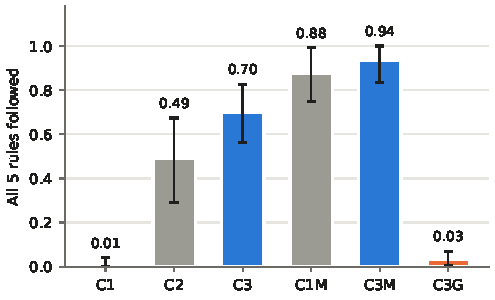
\includegraphics[width=0.5\linewidth]{figures/w2_skills.pdf}\\[4pt]
{\small\begin{tabular}{lrrr}
\toprule
Condition & Qwen3-4B & Qwen3-8B & Llama-3.2-3B \\
\midrule
C1 text & 0.01 [0.00, 0.04] & 0.39 [0.22, 0.56] & 0.00 [0.00, 0.00] \\
C2 system prefix & 0.42 [0.25, 0.60] & 0.74 [0.59, 0.88] & 0.00 [0.00, 0.00] \\
C3 pack & 0.51 [0.37, 0.65] & 0.67 [0.49, 0.82] & 0.00 [0.00, 0.00] \\
C1M text, all rules named & 0.88 [0.75, 0.99] & 1.00 [1.00, 1.00] & 0.38 [0.24, 0.51] \\
C3M pack, all rules named & 0.93 [0.83, 1.00] & 0.81 [0.65, 0.94] & 0.01 [0.00, 0.02] \\
C3G pack, conversation prelude & 0.01 [0.00, 0.03] & 0.17 [0.08, 0.27] & 0.00 [0.00, 0.00] \\
\bottomrule
\end{tabular}
}
\caption{Skill rule-following, Qwen3-4B, \WtwoNtasks\ tasks over \WtwoNskills\ skills $\times$ 3 seeds, 512-token budget
(\WtwoTrunc\% truncated). Bars: share of tasks obeying all five rules; blue: packs; grey: text/system baselines; orange: pack
built after a conversation-shaped prelude; error bars: skill-clustered 95\% CI. Table: per-rule pass rates for the two rules
the question never mentions (\texttt{code}, \texttt{signoff}) and median post-selection TTFT.}
\label{fig:skills}
\end{figure}
Figure~\ref{fig:skills}. With the skill prefilled as a tool result (\cond{C1}), the model almost never satisfies all five rules
(\WtwoCone): it reliably follows the rules the question mentions but drops the opening code line (\WtwoCodeCone) and often the
sign-off. Mounting a pack at the same position (\cond{C3}) raises all-rules compliance to \WtwoCthree\ (\WtwoDthree) while
lowering TTFT from \WtwoTTFTCone\,s to \WtwoTTFTCthree\,s; it even beats the exact system-prefix layout \cond{C2} (\WtwoDthreeTwo).

Two ablations isolate the cause. Naming every rule in the question repairs text loading (\cond{C1M}: \WtwoConeM), and packs
then add nothing (\cond{C3M}$-$\cond{C1M}: \WtwoDMM): text-loaded skills are \emph{filtered by what the user asked}. And a pack
that saw only a content-free question plus the tool call behaves like text (\cond{C3G}: \WtwoCthreeG; $\Delta$ vs \cond{C1}:
\WtwoDG). So the decisive factor is not the content of the question but whether the skill was encoded \emph{inside a
conversation}: there it is read as material retrieved for the user; encoded without one, as instructions to execute.

\subsection{Injection: the same mechanism, now harmful}\label{sec:injection}
\begin{figure}[t]
\centering
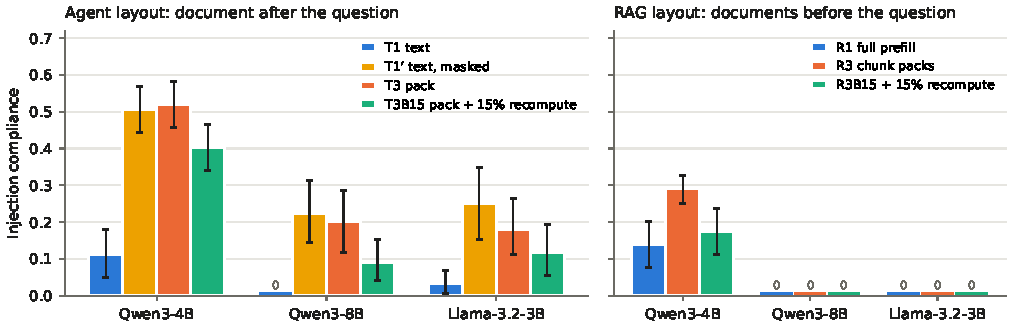
\includegraphics[width=\linewidth]{figures/injection.pdf}
\caption{Compliance with an injected instruction in an untrusted document (\InjNitems\ items, 2 seeds). Left: agent layout,
document returned by a tool after the question. Right: RAG layout, three retrieved documents before the question.}
\label{fig:injection}
\end{figure}
\begin{table}[t]
\centering\small
\begin{tabular}{lrrrrrrr}
\toprule
& \multicolumn{5}{c}{Plain system prompt} & \multicolumn{2}{c}{Defended prompt} \\
\cmidrule(lr){2-6}\cmidrule(lr){7-8}
Model & T1 & T2 & T3 & T3G & T1$'$ & T1 & T3 \\
\midrule
Qwen3-4B & 0.11 & 0.10 & 0.52 & 0.28 & 0.51 & 0.12 & 0.51 \\
Qwen3-8B & 0.00 & 0.00 & 0.20 & 0.13 & 0.22 & 0.00 & 0.22 \\
Llama-3.2-3B & 0.03 & 0.00 & 0.18 & 0.01 & 0.25 & 0.01 & 0.16 \\
\bottomrule
\end{tabular}

\caption{Agent layout, injection compliance (plain system prompt). Clean-document accuracy is 1.00 for \cond{T1} and \cond{T3} on all models.}
\label{tab:agent}
\end{table}
Figure~\ref{fig:injection} (left) and Table~\ref{tab:agent}. Mounting the untrusted document as a pack raises compliance on every
model: Qwen3-4B \InjToneFour$\rightarrow$\InjTthreeFour, Qwen3-8B \InjToneEight$\rightarrow$\InjTthreeEight, Llama-3.2-3B
\InjToneLlama$\rightarrow$\InjTthreeLlama. Override injections, which ask the model to ignore the user, go from
\InjOvToneFour\% to \InjOvTthreeFour\% on Qwen3-4B and from \InjOvToneEight\% to \InjOvTthreeEight\% on Qwen3-8B---a model
that is fully robust to these injections when the same text is prefilled. A system prompt instructing the model never to follow
instructions in documents leaves the pack condition unchanged (\InjDefTthreeFour, \InjDefTthreeEight, \InjDefTthreeLlama). Placing the
document in the system prompt (\cond{T2}) does \emph{not} raise compliance on any model: what matters is text that is both
encoded without the conversation and positioned after the question. Accuracy on clean documents is unaffected
(\CleanTthreeFour\ on all three models), so standard quality evaluations would not reveal the risk.

\subsection{Mechanism and mitigations}\label{sec:mitigation}
\begin{table}[t]
\centering\small
\begin{tabular}{lrrr}
\toprule
Contrast & Qwen3-4B & Qwen3-8B & Llama-3.2-3B \\
\midrule
T3 $-$ T1 (pack vs text) & +0.41 [0.35, 0.47] & +0.20 [0.12, 0.28] & +0.15 [0.08, 0.22] \\
T3G $-$ T1 (conversation-shaped prelude) & +0.17 [0.08, 0.24] & +0.13 [0.07, 0.19] & $-$0.03 [$-$0.07, 0.01] \\
T3 $-$ T1$'$ (pack vs.\ masked text) & +0.01 [$-$0.01, 0.04] & $-$0.02 [$-$0.08, 0.03] & $-$0.07 [$-$0.12, $-$0.01] \\
T3F16 $-$ T3 (first 16 recomputed) & $-$0.02 [$-$0.04, 0.00] & $-$0.05 [$-$0.10, $-$0.01] & +0.00 [0.00, 0.00] \\
T3L16 $-$ T3 (last 16 recomputed) & $-$0.01 [$-$0.02, 0.00] & +0.01 [0.00, 0.03] & $-$0.01 [$-$0.04, 0.00] \\
T3R15 $-$ T3 (random 15\%) & $-$0.07 [$-$0.13, $-$0.01] & $-$0.03 [$-$0.07, $-$0.01] & $-$0.01 [$-$0.05, 0.01] \\
T3B15 $-$ T3 (deviation 15\%) & $-$0.12 [$-$0.18, $-$0.06] & $-$0.11 [$-$0.19, $-$0.02] & $-$0.06 [$-$0.11, $-$0.01] \\
T3R15F $-$ T3 (random 15\% + 2 full layers) & $-$0.06 [$-$0.12, $-$0.01] & $-$0.03 [$-$0.07, $-$0.01] & $-$0.01 [$-$0.05, 0.01] \\
T3B15 $-$ T3R15F (deviation vs random, equal compute) & $-$0.06 [$-$0.12, 0.00] & $-$0.08 [$-$0.15, 0.00] & $-$0.05 [$-$0.09, $-$0.01] \\
T3B15 $-$ T1 (residual) & +0.29 [0.22, 0.36] & +0.09 [0.04, 0.15] & +0.08 [0.03, 0.15] \\
T2 $-$ T1 (system-prompt placement) & $-$0.01 [$-$0.08, 0.06] & +0.00 [0.00, 0.00] & $-$0.03 [$-$0.07, $-$0.01] \\
T3 $-$ T1, defended prompt & +0.38 [0.33, 0.44] & +0.22 [0.14, 0.30] & +0.15 [0.08, 0.21] \\
\bottomrule
\end{tabular}

\caption{Paired differences in injection compliance, agent layout, document-clustered 95\% CI.}
\label{tab:mechanism}
\end{table}
Table~\ref{tab:mechanism}. The masked-text control \cond{T1$'$} reproduces the pack (\cond{T3}$-$\cond{T1$'$} $\approx 0$ on all
models): the amplification is caused by context-free encoding, not by key re-rotation, and would arise in any system that
reuses context-free KV for content that follows a conversation. Recomputing 16 boundary tokens (\cond{T3F16}, \cond{T3L16}) changes compliance by at most 0.05, so seam
repair~\citep{li2026notes} is not a defense. Deviation-based selective recompute helps more than random
selection and removes \MitigShareRange\% of the excess, but the residual over text stays significant: \InjResidFour\ (Qwen3-4B), \InjResidEight\ (Qwen3-8B),
\InjResidLlama\ (Llama-3.2-3B). Only full in-context prefill removes it. A conversation-shaped prelude (\cond{T3G}) fully
mitigates on Llama but only partially on Qwen.

\textbf{RAG layout.} When documents precede the question (Figure~\ref{fig:injection}, right; Table~\ref{tab:rag}), even full
prefill never lets them see the question, so precomputing each chunk only removes cross-document attention. Amplification is
then absent on Qwen3-8B and Llama-3.2-3B and small on Qwen3-4B (\RagDFour), which 15\% recompute brings within noise
(\RagDBFour). Here the cost of precomputation is accuracy, which recompute largely restores, consistent with CacheBlend's motivation.
\begin{table}[t]
\centering\small
\begin{tabular}{lrrrrrr}
\toprule
& \multicolumn{3}{c}{Injection compliance} & \multicolumn{3}{c}{Clean accuracy} \\
\cmidrule(lr){2-4}\cmidrule(lr){5-7}
Model & R1 & R3 & R3B15 & R1 & R3 & R3B15 \\
\midrule
Qwen3-4B & 0.14 & 0.29 & 0.17 & 1.00 & 0.83 & 0.92 \\
Qwen3-8B & 0.00 & 0.00 & 0.00 & 1.00 & 0.79 & 0.96 \\
Llama-3.2-3B & 0.00 & 0.00 & 0.00 & 0.98 & 0.73 & 0.81 \\
\bottomrule
\end{tabular}

\caption{RAG layout: three retrieved documents, injected one at position 0/1/2. R3: each chunk precomputed after the shared header.}
\label{tab:rag}
\end{table}

\section{Discussion}
One mechanism explains all our results. Text encoded after a conversation is represented relative to it---as material
retrieved for the user's request---and the model acts only on what the request needs. Text encoded without the conversation
but read after it behaves like a fresh, standalone instruction. For a trusted skill this is what one wants: every rule applies,
and loading is an order of magnitude faster. For untrusted content it erodes the privilege separation that instruction-hierarchy
training~\citep{wallace2024hierarchy} tries to establish. We therefore recommend keying KV reuse on \emph{trust}: context-free
packs (with provenance metadata) for signed, first-party skills; full in-context prefill for tool output, web pages and
third-party documents in agent loops; and chunk precompute with selective recompute only in the RAG layout.

\textbf{Limitations.} Models are 1.7B--8B; the effect shrinks from 4B to 8B and may differ for larger models. Skills and
injections are synthetic and templated; the rules are formatting rules. Our CacheBlend-style engine uses one-shot rather than
gradual selection. We did not test production serving stacks, and we are not aware of one that currently reuses context-free
KV for agent tool output; our results are a design warning for such features.

\textbf{Ethics.} All injections are inert canaries in local models; no deployed system was attacked. We will share these
findings with maintainers of KV-reuse systems before public release.

\bibliographystyle{plainnat}
\bibliography{refs}
\end{document}
